\documentclass[parskip=half]{scrartcl}
\usepackage{fontspec}
\usepackage[ngerman]{babel}
\usepackage{hyperref}
\usepackage{csquotes}

% nicht einmal notwendig, ist eh standard
%\fontspec{Latin Modern Roman}

\author{Simon~Becker, Marek~Kubica\\TU~München}
\title{Die Geschichte der Rechnerarchitektur\\
Sommersemester 2013\\
Verarbeitung von Lochkarten: Hollerith und die D11}

\date{22.~März~2013}

\begin{document}
\maketitle

\begin{abstract}

Die Zusammenfassung ist eine Kurzfassung des Artikels. Sie sollte
auch getrennt vom restlichen Text verständlich sein
und bildet eine abgeschlossene Einheit. Insbesondere sollten keine
Verweise auf andere Abschnitte
oder das Literaturverzeichnis gemacht werden. Auf eine Einleitung
und einen Schluß kann hier verzichtet werden, um Platz zu sparen.

Ziel der Zusammenfassung ist in erster Linie, den Lesern die Wahl
zu erleichtern, welche Artikel sie lesen sollen. Folge: ist die
Zusammenfassung schlecht, schwammig oder langweilig, wird der
Artikel seltener gelesen.
\end{abstract}

\section{Einleitung}
\label{sec:einleitung}

Um die von Hollerith geprägte Geschichte der Lochkarten zu verstehen ist es
zunächst einmal notwendig, den Begriff des Tabellierens zu klären.

Beim Tabellieren werden nicht zwingend vorsortierte Daten nach bestimmten
Kriterien ausgewertet und danach für weitere Verarbeitung sortiert abgelegt.
Dieser Vorgang ist notwendig um Datensätze nach bestimmten, gegebenfalls sogar
voneinander abhängigen Kriterien auswerten zu können. So kann durch das
Tabellieren von Volkszählungsdatensätzen bestimmt werden wie viele Einwohner
eines Landes Staatsbürger sind und wieviele Immigranten. Die Immigranten etwa
können daraufhin nach weiteren Kriterien analysiert werden, wie etwa
Ursprungsland oder Einwanderungsjahr.

Solch eine Verarbeitung von Daten ist für Bevölkerungsstatistiken interessant,
kann aber auch verwendet werden um Firmendaten zu verarbeiten, wie etwa die
Arbeitszeiten von Angestellten, die Einnahmen von Kundenverträgen, also
allgemein vieles was unter dem Namen Buchhaltung zu finden ist.

Dabei ist zu beachten, dass Tabellieren nicht zwingend eine Maschine
vorraussetzt: vor Holleriths Tabelliermaschinen wurde dieser Vorgang von Hand
ausgeführt, Hollerith hat diese mechanische Tätigkeit jedoch automatisiert.

Heutzutage sind Tabelliermaschinen selbst ausgestorben, aber ihre Funktion ist
in Software wie Tabellenkalkulationen und Datenbanken noch bis heute
unverzichtbar.

\section{Herman Hollerith}
\label{sec:hollerith}

Herman Hollerith wurde am 29.~Februar 1860 in Buffalo, New York geboren, als
Sohn deutschstämmiger Einwanderer. Dies bedeutet auch, dass Hollerith selbst
US-Amerikaner war jedoch mit einem deutsch klingenden Namen. Diese
Unterscheidung ist später für die Dehomag bedeutend, aber für Hollerith
bedeutet dies erstmal dass seine Geschichte hauptsächlich in den USA spielt.

Hollerith studierte Minenbau und erlangte 1879 einen \enquote{Engineer of
Mines}-Abschluss, auf den 1880 sein Ph.D. folgte.

% TODO: heirat
% todo familie

% todo am MIT

1884 arbeitete Hollerith in einem Zensusbüro. Dort kam er mit der Realität von
Volkszählungen und ihrer Auswertung in Kontakt. Damals verliefen Voklszählungen
so dass die Bürger Fragebögen ausfüllen mussten auf denen eine Reihe von Fakten
abgefragt wurde. Diese Fragebögen wurden später eingesammelt und an zentraler
Stelle, im Zensusbüro, ausgewertet.

Dabei wurden die Datensätze durchgegangen, nach bestimmten Kriterien
ausgewertet und sortiert. Um komplexere Kriterien auszuwerten mussten die
Datensätze mehrmals durchlaufen werden, Beispiele dafür sind etwa wie viele
Immigranten sind Selbstständig (auswertung nach Anzahl der Immigranten, danach
diese Daten nach Selbstständigen auswerten) oder wie viele Weiße wurden 1880
geboren (Auswertung nach Hautfarbe und danach nochmals nach Geburtsjahr).

Dieses Verfahren ist effektiv aber erfordert viel Aufwand die Datensätze
durchzugehen und richtig einzusortieren. Hollerith erkannte, dass diese Arbeit
eine im Grunde mechanische war und dass diese durch Maschinen unterstützt
werden könne.

\subsection{Lochkarten als Datensätze}
\label{sec:lochkarten}

Hollerith suchte nach einer Möglichkeit die Datensätze zu repräsentieren als
ihm bei einer Zugfahrt die Idee kam eine Lochkarte zu verwenden. Inspiriert
wurde er durch sein Zugticket, welches ein. \enquote{Punch Photograph} war. Die
Idee hinter einem \enquote{Punch Photograph} war, dass die Eigenschaften des
Ticketbesitzers auf einem Bogen Papier mit Löchern eingestanzt werden, so dass
dieses Ticket nicht mehr ohne weiteres Übertragbar ist. Dabei werden
Eigenschaften wie Geschlecht, ungefähres Aussehen, ungefähres Alter sowie
Strecke und Fahrtzeit notiert.

Auf diese Weise konnte man die Lochkarte einer Person als einzelnen Datensatz
ansehen, in dem verschiedene Daten über eine Person durch die Anordnung der
Löcher enkodiert werden können. Tatsächlich nutzte Hollerith in der Anfangszeit
eine Handstanze wie sie Fahrkartenkontrolleure eingesetzt haben, so dass die
Löcher sich an dem Rand der Karte befanden.

\subsection{1890}
\label{sec:1890}

Im 19ten Jahrhundert wurde in den USA die Volkszählung alle zehn Jahre durch
das Zensusbüro organisiert und ausgeführt. Für die Durchführung einer solchen
Volkszählung wurde vor der Zählung der aktuelle Stand der Technik evaluiert und
es fand eine Ausschreibung statt.

Hollerith hat für die Ausschreibung für die Volkszählung 1890 ein komplettes
System erarbeitet:

\begin{itemize}
  \item Die Daten wurden über eine Lochkartenstanze eingegeben. Dabei wurde
    die Lochkarte in die Stanze oben eingelegt. Die verschiedenen Werte die
    eingegeben werden konnten, waren auf einer Vorlage mit Löchern unten in
    der Stanze notiert, so dass der Operator einen Hebel über die Vorlage
    bewegte und den Hebel in die betreffenden Löcher der Vorlage vertiefte.
    Dabei wurde gleichzeitig in die oben eingelegte Lochkarte das entsprechende
    Loch eingestanzt. Der Vorgang ist rein mechanisch. Die 1890 verwendeten
    Lochkarten waren unbedruckt, für das menschliche Ablesen der Karten
    lieferte Hollerith Vorlagen mit, die über die Lochkarten gelegt werden
    konnten~\cite{austrian1982herman}.
  \item Die so gelochten Karten wurden in die Tabelliermaschine eingelesen,
    indem die Karte in die Lesevorrichtung eingelegt wurde und der Hebel dieser
    Vorrichtung nach unten gedrückt wurde. Dies führte dazu dass die Kontakte
    im Hebel durch die Löcher in der Lochkarte Schaltkreise schlossen die zum
    inkrementieren der jeweiligen, für die Löcher der Karte zugehörigen Werte
    führten. Die Tabelliermaschine selbst enthielt Reihen von Zähluhren, die
    diese Werte anzeigten und am Ende vom Operator abgelesen
    wurden~\cite{deutschesmuseum}.
  \item Nachdem die Karte eingelesen wurde, hat die Tabelliermaschine in der
    Sortiermaschine ein Fach geöffnet, in die die Lochkarte vom Operator
    reingelegt wurde.
\end{itemize}

Neben dem System von Hollerith wurden auch zwei weitere Systeme, von William C.
Hunt sowie Charles F. Pidgin, getestet. Als Testdaten wurde eine Untermenge der
tatsächlichen Daten des vorhergehenden Zensus von 1880 verwendet. Die
Untermenge enthielt Daten der Zählung von vier Auszählungsbezirken von St.
Louis und beschrieb 10.491 Einwohner. Getestet wurden \emph{Transkription}
(also das Aufnehmen der Daten in Lochkartenformat) sowie \emph{Verarbeitung}
(also das Tabellieren)~\cite{austrian1982herman}.

\begin{itemize}
  \item Hollerith-System: 72~Stunden, 27~Minuten für die Transkription sowie
    5~Stunden 28~Minuten für die Verarbeitung
  \item Hunt-System: 144~Stunden, 25~Minuten für Transkription, 55~Stunden,
    22~Minuten für Verarbeitung
  \item Pidgin-System: 110~Stunden, 56~Minuten für Transkription,
    44~Stunden, 41~Minuten für Verarbeitung
\end{itemize}

Aufgrund der deutlich schnelleren Arbeitsweise des Hollerith-Verfahrens,
insbesondere der Tabelliermaschine, war die Verwendung in der kommenden
Volkszählung beschlossen.

\subsection{1900}

\subsection{Kommerzielle Vermarktung}

\section{Dehomag D11}
\label{sec:d11}


\section{Eine deutsch-amerikanische Erfolgsgeschichte}

Wenn man sich über den Amerikaner Herman Hollerith und seine Erfindung die
Hollerith-Lochkarte informiert und welchen Einfluss diese Erfindung auf
Deutschland hatte, stößt man früher oder später auf die deutsche Firma
\enquote{Dehomag}. In diesem Abschnitt soll der Werdegang der Dehomag erläutert
werden und weshalb sie bedeutend  für die Entwicklung der Lochkartentechnik
ist.

\subsection{Anfangszeit der Dehomag}

Im November 1910 wurde die \enquote{Deutsche Hollerith-Maschinen Gesellschaft
mbH} oder kurz \enquote{Dehomag} von Willy Heidinger in Berlin
gegründet~\cite{dingwerth}. Das erste Werk hatte man in Villingen. Die Dehomag
produzierte Locher und Sortierer für die Hollerith-Lochkarten und
Tabelliermaschinen. Aufgrund der Inflation konnte die Dehomag während des
ersten Weltkrieges ihre Lizenzgebühren an die \enquote{Computing Tabulating
Recording Company} (CTR) nicht mehr bezahlen.  Daraufhin kaufte CTR 1922 90\%
der Firmenanteile der Dehomag auf~\cite{restloseErfassung}. 1924 wurde die CTR
übrigens in \enquote{International Business Machines Corporation} (IBM)
umbenannt. Nachdem das Werk in Villingen aufgelöst worden war, wurde ab 1927 in
Sindelfingen produziert. Im Januar 1934 wurde dann in
\enquote{Berlin-Lichterfelde mit über 400 Mitarbeitern ein eigenes
Produktionswerk sowie eine neue Hauptverwaltung}~\cite{dingwerth} der Dehomag
eröffnet.

\subsection{Von Dehomag zu IBM}

Nach der Erfindung der D11 konnte die Dehomag in den folgenden Jahren sowie
während des zweiten Weltkrieges Gewinne erwirtschaften. Allein in den ersten
acht Jahren wurden mehr als 1100 Tabelliermaschinen vom Typ D11
ausgeliefert~\cite{Kist95}. Die Dehomag trug entscheidend zur Verbreitung der
D11 in den Betrieben bei. Die Firma wurde stetig größer und 1940 war sie
bereits in Deutschland und Österreich in 59 Städten vertreten und beschäftigte
mehr als 2500 Mitarbeiter~\cite{dingwerth}. 1960 wurde schließlich die
letzte D11 gebaut und obwohl es die ersten programmierbaren Rechner gab, waren
zu der Zeit noch ungefähr 200 D11 Maschinen in Betrieb. Allerdings wurden die
D11 in den nächsten Jahren immer weniger genutzt und durch Computer ersetzt.
Heute steht eine der letzten restaurierten D11 Tabelliermaschinen in München im
Deutschen Museum~\cite{Kist95}.

Zu den Kunden der Dehomag gehörten unter anderem statistische Ämter, die
Industrie und während des Krieges die Wehrmacht sowie die Schutzstaffel der
Nationalsozialisten. Aufgrund des Krieges konnte IBM mit seiner Tochterfirma
Dehomag nur in neutralen oder von deutschen Truppen besetzten Ländern
zusammenarbeiten. Erst nach dem Ende des Krieges 1945 wurde IBM wieder in
Deutschland geschäftlich tätig. Im Jahr 1949 wurde die Dehomag dann in
\enquote{Internationale Büro-Maschinen Gesellschaft mbH} (IBM) umbenannt,
woraus später die \enquote{IBM Deutschland GmbH} wurde~\cite{sendler}.
Noch heute ist IBM in ganz Deutschland vertreten und gehört zu den führenden
Unternehmen im IT- Bereich. Es ist eine deutsch-amerikanische
Erfolgsgeschichte.

\section{Weiterentwicklung der D11}

Die Dehomag Tabelliermaschine D11 verkaufte sich wie erwähnt sehr gut, aber war
nicht die letzte Maschine in der Geschichte der Lochkartentechnik. Beim Einsatz
der D11 Maschine kristallisierten sich die Kritikpunkte eines unzureichenden
Zeichenvorrates, zu langsamer Druckgeschwindigkeit und zu geringer
arithmetischer Leistung heraus~\cite{sandner}. Im Jahr 1949 kam mit der
Buchungsmaschine IBM 407 eine Weiterentwicklung auf den Markt, die ein
neuartiges Druckwerk beinhaltete. Die Neuerung war ein sich nur vorwärts
drehendes, elektromagnetisch gesteuertes Rad. Dieses Rad wurde Typenrad genannt
und war der Träger des Zeichensatzes. Zusätzlich zum Alphabet und den
einstelligen Zahlen enthielt das Typenrad elf Sonderzeichen, welche nicht
chronologisch angeordnet waren (siehe \autoref{fig:typenrad}). Die Aufhängung
des Typenrades besorgte eine Schwinge, wodurch das Typenrad selbst zum Hammer
wurde. Mit dieser Technik konnte die Druckgeschwindigkeit erhöht und ein
qualitativ gutes Druckbild durch exakte Typenpositionierung gewährleistet
werden~\cite{sandner}. Ein weiterer Vorteil der IBM 407 war, dass die
Operationen auf den Lochkarten im Gegensatz zu vorher mit einem einzigen
Maschinenzyklus durchgeführt werden konnten~\cite{Boyell}. Aufgrund der
Möglichkeit der neuen Zeichenkombinationen wurden gleichzeitig neue
Kartenlocher und Prüfer entwickelt, damit die neue Technik eingesetzt werden
konnte.

\begin{figure}[h]
  \centering
  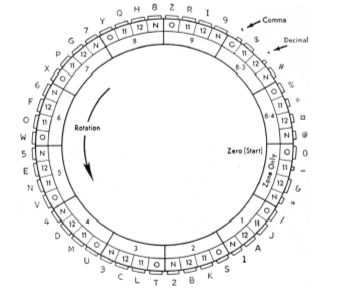
\includegraphics{typenrad}
  \caption{Schematisch dargestelltes Typenrad der IBM 407 von der Seite~\cite{sandner}}
  \label{fig:typenrad}
\end{figure}

Die Entwicklung und Produktion der IBM 407 fand bei IBM in der USA statt und
aufgrund der Währungsrelation war die Monatsmiete für eine IBM 407 in Europa
deutlich teurer als die Miete für ein Dehomag D11~\cite{sandner}. Aus diesem
Grund war die D11 in Europa verbreiteter. Anfang der 1950er Jahre kam mit der
Tabelliermaschine IBM 421 eine wichtige Weiterentwicklung für den europäischen
Markt heraus (siehe \autoref{fig:IBM421}). Diese besaß eine umfassende
Programmsteuerung und konnte an die gewünschten Arbeiten ihrer Anwender
angepasst werden~\cite{deutschesMuseum}. Eine Alphabetzeile konnte ebenfalls
wie bei der IBM 407 in einem Maschinenzyklus gedruckt werden. Anstatt dem sich
vorwärts drehendem Typenrad wurde bei der IBM 421 wieder das
Typenstangendruckprinzip genutzt, wobei es für jede Typenstange eine neuartige
Antriebssteuerung gab. Die Produktion der IBM 421 fand bei IBM Frankreich und
bei der in IBM Deutschland umbenannten Dehomag statt. \enquote{Aufgrund ihrer
Universalität war die 421 außer in Europa ein bis Nahost, Fernost, Afrika und
Südamerika gefragtes Produkt.}~\cite{sandner}.

\begin{figure}[h]
  \centering
  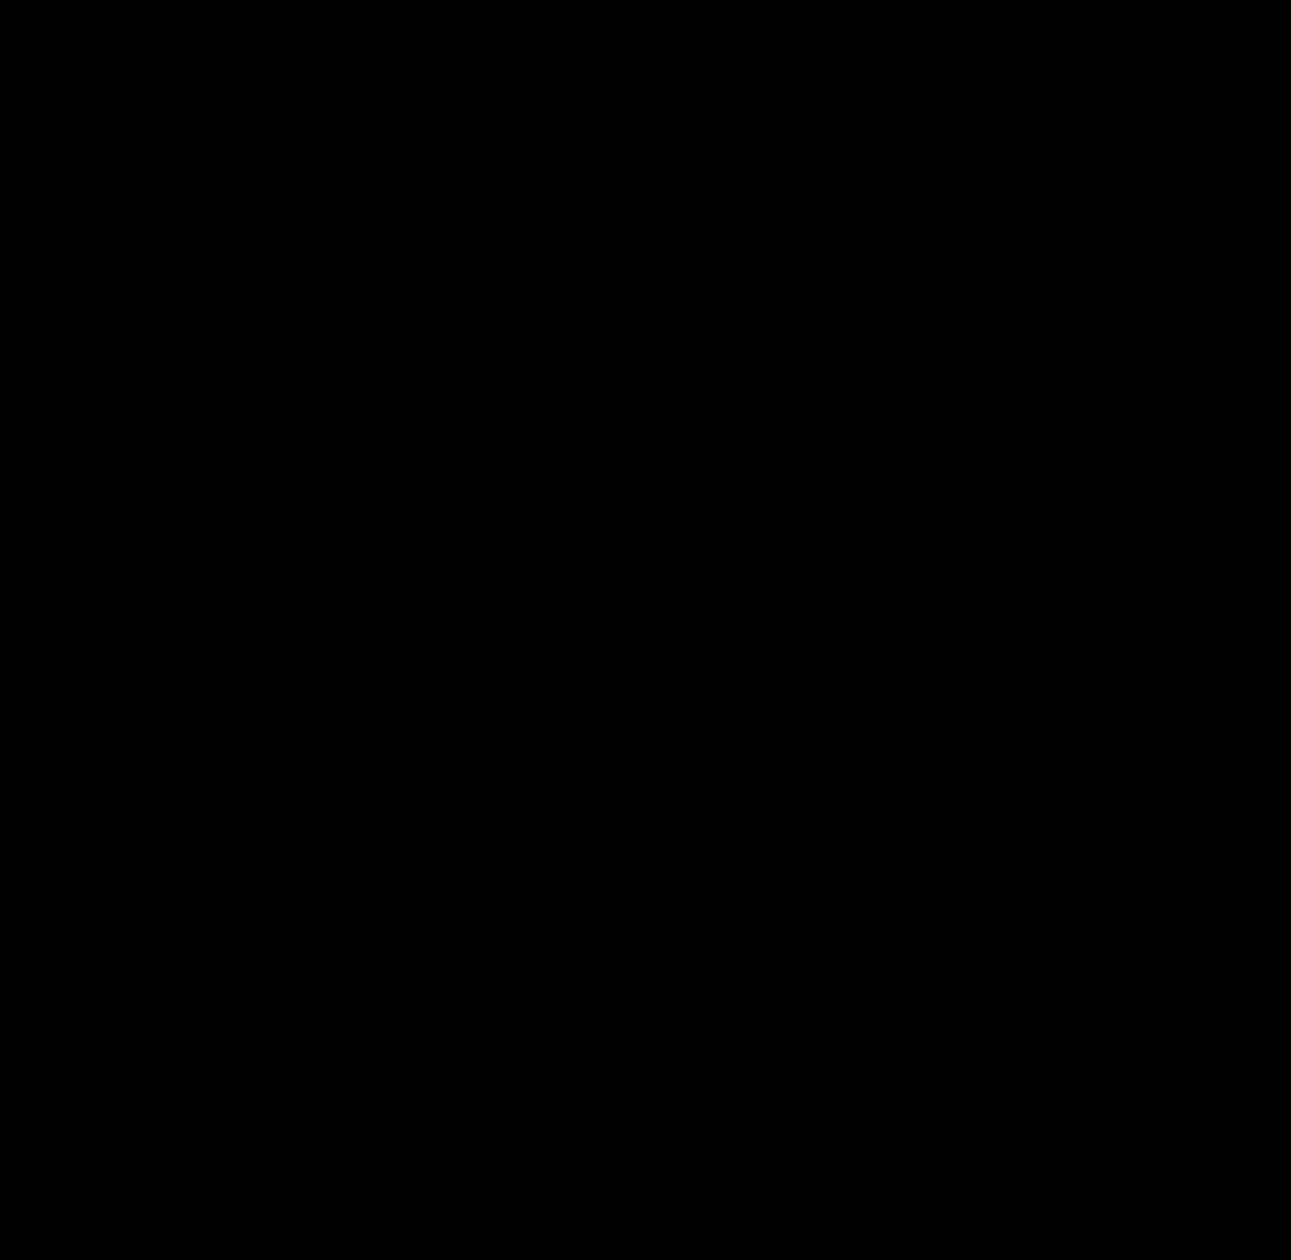
\includegraphics{IBM421}
  \caption{Tabelliermaschine IBM 421~\cite{sandner}}
  \label{fig:IBM421}
\end{figure}

\section{Magnetische Speicherung ersetzt Lochkarte als Speichermedium}

Obwohl die IBM 421 in vielen Ländern zum Einsatz kam und \enquote{Anwender mit
um die 10 Tabelliermaschinen in der zentralen
Lochkartenabteilung}~\cite{sandner} keine Seltenheit waren, gehörte die IBM 421
zu den letzten Weiterentwicklungen. Der Grund dafür war die Verwendung der
magnetische Speicherung von binären Daten, wodurch die Lochkarten in den 1960er
Jahren als Medium für Massenspeicherung abgelöst wurden~\cite{gronau2009}. Bei
dieser Speichertechnik wird beim Schreiben eine Polaritätsänderung der
Ferritteile in der  ferromagnetischen Oberfläche erzeugt. Je nachdem, ob der
Bereich Richtung Nord- bzw. Südpol zeigt, wird beim Lesen die Richtung des
Magnetfeldes als 0 oder 1 interpretiert~\cite{gronau2009}. Für die magnetische
Speicherung können Bänder, Karten oder Platten genutzt werden. Das Prinzip der
Magnetspeicherung findet auch bei den heutigen Festplatten Anwendung.

Abschließend werden die Vor- und Nachteile dieser neuen Speichertechnik
genannt. Ein Vorteil von magnetischen Datenträgern gegenüber von Lochkarten ist
die Wiederverwendbarkeit. Alte Daten können gelöscht und neu überschrieben
werden. Außerdem sind die Kosten pro Gigabyte bei magnetischen Datenträgern
günstiger als bei den Lochkarten~\cite{Dee}. Aufgrund physikalischer und
technischer Grenzen hat der magnetisierte Bereich eine bestimmte Größe, weshalb
das Speichervolumen eines solchen Datenträger endlich ist. Ein Nachteil
magnetischer Datenträger ist somit, dass sie nicht beliebig klein sein können.

\section{Lochkarten im digitalen Zeitalter}

In diesem Abschnitt sollen Beispiele und Bereiche gezeigt werden, in denen auch
noch in dieser technisch weit vorangeschrittenen Zeit Lochkarten oder das
Prinzip der Lochkartentechnik zum Einsatz kommen. Die USA benutzt
beispielsweise vereinzelt in ihren Wahlautomaten Lochkarten, um ein schnelles
auswerten der Stimmen zu gewährleisten. So gaben bei der Präsidentschaftswahl
im Jahr 2000 die Bürger der Stadt Palm Beach im Bundesstaat Florida ihre Stimme
durch das Stanzen eines Loches in eine Lochkarte ab~\cite{simons}. Probleme bei
der Auswertung der Stimmen in Florida ließen die Lochkarten in Verruf geraten
und schließlich führte ein Urteil des Obersten Gerichtshof der Vereinigten
Staaten zum Wahlsieg von George W. Bush. Dennoch wurde bei der bisher letzten
US-Wahl 2012 \enquote{per Brief- oder Online-Wahl und - wie in manchen Gegenden
in Idaho - zum Teil auch noch mit Lochkarten}~\cite{keinVerfasser} abgestimmt.
Bei dieser Wahl gab es keine bekannten negative Zwischenfälle. Des Weiteren
existiert in der Stadt Conroe in Texas die Firma \enquote{Sparkler Filters},
die ihre Buchhaltungsaufgaben bis heute mit der Tabelliermaschine Sparklers IBM
402 auf Hollerith-Lochkarten ausführt~\cite{edwards}.

IBM benutzt zwar keine Tabelliermaschinen mehr, verwendet aber in seinem
Projekt \enquote{Millipede} das Grundprinzip der Lochkarten. Bei diesem Projekt
handelt es sich um eine Speichertechnik, welche im Nanometerbereich angewendet
wird.  Mit winzigen Messnadeln können Bits in einen Polymerfilm geschrieben,
gelesen oder gelöscht werden~\cite{binnig}. Eine Vertiefung im
Polymerfilm wird dabei als 1 und die unveränderte Oberfläche als 0
interpretiert. Der Unterschied zu herkömmlichen Lochkarten ist somit neben der
Größe die Möglichkeit Bits zu löschen und zu überschreiben. Mit dieser Technik
können bis zu ein Terabyte pro Quadratzoll (in²) gespeichert werden, wobei ein
Quadratzoll der Fläche von 6,4516cm² entspricht~\cite{binnig}. Die
Lese- und Schreibgeschwindigkeit kann durch Nutzung von mehreren parallel
arbeitenden Messnadeln optimiert werden.

Diese aufgezeigten Beispiele sind allerdings die Ausnahme, denn die
Lochkartentechnik ist in der heutigen Zeit veraltet und in der Computertechnik
nicht mehr von Bedeutung. Ein Zahlenbeispiel wird den technischen Fortschritt
im Bereich der Datenspeicherung belegen: Die am häufigsten verbreiteten
Lochkarten besaßen 80 Spalten und konnten somit 80 Byte speichern. Rechnet man
das auf eine 120 GB Festplatte hoch, so kommt man auf eine Anzahl von über 1,6
Milliarden Lochkarten, die die selbe Speicherkapazität wie diese Festplatte
besitzen~\cite{roeltgen}. Mittlerweile gibt es bereits Festplatten mit sehr
viel mehr als 120 GB Speicher.

\section{Fazit}

\bibliographystyle{plain}
\bibliography{ausarbeitung}

\end{document}
